%----------------------------------------------------------------------------------------
%	PACKAGES AND OTHER DOCUMENT CONFIGURATIONS
%----------------------------------------------------------------------------------------

% \documentclass[10pt, a4paper, twocolumn]{article} % 10pt font size (11 and 12 also possible), A4 paper (letterpaper for US letter) and two column layout (remove for one column)
\documentclass[12pt, a4paper]{article} % 10pt font size (11 and 12 also possible), A4 paper (letterpaper for US letter) and two column layout (remove for one column)

\input{preamble.tex} % Specifies the document structure and loads requires packages

\usepackage{amsmath}

%----------------------------------------------------------------------------------------
%	ARTICLE INFORMATION
%----------------------------------------------------------------------------------------

\title{Protocol Synthesis in the Dynamic Gossip Problem} % The article title

\author{
	\authorstyle{Leo Poulson}
	\newline\newline % Space before institutions
}


\date{\today} % Add a date here if you would like one to appear underneath the title block, use \today for the current date, leave empty for no date

%----------------------------------------------------------------------------------------

\begin{document}

\maketitle % Print the title

\thispagestyle{firstpage} % Apply the page style for the first page (no headers and footers)

%----------------------------------------------------------------------------------------
%	ABSTRACT
%----------------------------------------------------------------------------------------
% \lettrineabstract{Project Summary; a 200-300 word outline of what your project will be. The summary might be comprised of your project's motivation, a comment on the current state of the art and its limitations, a summary of what you will do and how you will evaluate your contribution. }

%----------------------------------------------------------------------------------------
%	ARTICLE CONTENTS
%----------------------------------------------------------------------------------------

\section{Dynamic Epistemic Logic}

\subsection{Epistemic Logic}

Epistemic Logic is a logic for the study of knowledge for a set of agents $I$ who want to reason about a set of propositions $\Lambda$. We recursively define the language of epistemic logic over this set of propositions, $\mc{L} \left(\Lambda\right)$, as follows;

\begin{equation}
    \phi ::= \top \mid p \mid \neg \phi \mid \phi \land \phi \mid K_i \phi 
\end{equation}

\noindent where $p \in \Lambda$ and $i \in I$. We can give $\mc{L} \left(\Lambda\right)$ a semantics using Kripke models as defined below. 

\hfill

A \textit{frame} for a set of agents $I$ is a tuple $\mc{M} = \left(U, R\right)$, where $U$ is a finite set of possible worlds and $R$ is a set of binary relations over $W$ indexed by an agent: $R_i \subseteq U \times U$ for $i \in I$.

A \textit{Kripke model} over a set of agents $I$ and a set of propositions $\Lambda$ is a tuple $\mc{M} = \left(U, R, \pi\right)$, where $\left(U, R\right)$ is a frame over $I$ and $\pi : U \to \mc{P}\left(\Lambda\right)$ is a valuation function; $\pi\left(w) \subseteq \Lambda\right)$ for every $w \in U$.

A \textit{pointed Kripke model} is just a pair $\left(\mc{M}, w\right)$, where $w$ is a world of $\mc{M}$.

\hfill

We can now give a semantics for $\mc{L}(\Lambda)$ on pointed Kripke models with the following inductive definition.

\begin{itemize}
    \item $(\mc{M}, w) \models \top \text{ always.}$
    \item $(\mc{M}, w) \models p \text{ iff } p \in \pi(w)$
    \item $(\mc{M}, w) \models \neg \phi \text{ iff not } (\mc{M}, w) \models \phi $
    \item $(\mc{M}, w) \models \phi \land \psi \text{ iff } (\mc{M}, w) \models \phi \text{ and } (\mc{M}, w) \models \psi$
    \item $(\mc{M}, w) \models K_i \phi \text{ iff } \left(\mc{M}, v\right) \models \phi \text{ for all } v \text{ such that } (w, v) \in R_i$.
\end{itemize}

\subsection{Dynamic Epistemic Logic}

In order to make our epistemic logic \textit{dynamic}, we need to have some formal way to reason about the dynamics of information, similarly to how Kripke models formalise static information. 

We can do this using \textit{action models}. Over a set of propositions $\Lambda$, an \textit{action model} is a tuple $\mc{E} = \left(E, R^{\mc{E}}, \pre, \post\right)$, where $E$ is a finite set of events, $R^\mc{E}$ is a set of relations $R_i \subseteq (E \times E)$ for each $i \in I$, $\pre : E \to \mc{L}(\Lambda)$ is a function assigning each event a formula called a \textit{precondition} and $\post : E \times \Lambda \to \mc{L}(\Lambda)$ is a function at each event assigns to each proposition a boolean formula called the \textit{postcondition}.

Given a Kripke model $\mc{M}$ and an action model $\mc{E}$, we define the \textit{update product} $\mc{M} \otimes \mc{E} := \left(U^{\otimes}, R^{\otimes}, \pi^{\otimes}\right)$ to be as follows:

\begin{itemize}
    \item $W^\otimes := \{\left(w, a\right) \in U \times A \mid \left(\mc{M}, w\right) \models \pre\left(a\right)\}$

    \item $R^\otimes_i := \{\left(\left(w, a\right), \left(v, b\right)\right) \mid R^\mc{M}_i wv \text{ and } R^\mc{A}_i ab\}$

    \item $\pi^\otimes((w, a)) := \{p\in\Lambda \mid \left(\mc{M}, w\right) \models \post\left(\left(a, p\right)\right) \}$
\end{itemize}

We define an \textit{action} in a similar way to a pointed Kripke model; they are simply a pair $\left(\mc{A}, a\right)$ where $a \in A$. To update a pointed Kripke model with an action model, we define $(\mc{M}, w) \otimes (\mc{E}, a) := (\mc{M} \otimes \mc{E}, (w, a))$.

\hfill

We now have everything we need to define the language of Dynamic Epistemic Logic (hereafter DEL). Given a vocabulary $\Lambda$, the language $\mc{L}_D(\Lambda)$ extends $\mc{L} \left(\Lambda\right)$ and is defined as:

\begin{align}
    \phi ::= \top \mid p \mid \neg \phi \mid \phi \land \phi \mid K_i \phi \mid [\mc{A}, a]\phi
\end{align}

\noindent where $p \in \Lambda$, $i \in I$ and $(\mc{A}, a)$ is an action.

We give identical semantics to $\mc{L}_D(\Lambda)$ as for $\mc{L}(\Lambda)$, except that we add in an operation for actions as follows.

\begin{itemize}
    \item $(\mc{M}, w) \models [\mc{A}, a]\phi \text{ iff } \mc{M}, w \models \pre (a) \text{ implies } \mc{M} \times \mc{A}, (w, a) \models \phi$.
\end{itemize}   

\section{The Gossip Problem}

We now want a use-case for DEL. The \textit{gossip problem} is an old problem about information sharing; we have a group of $n$ gossipers, each of whom know some piece of gossip that the others don't know. They communicate by telephone, and when one calls another, they tell each other everything they each know. Each gossiper may have the phone number of any number of other gossiper; they may only call another gossiper if they have their phone number. 

Naturally, this model isn't limited to people chatting on the phone; it could be generalised to distributed copies of a document that can be edited separately but need to be synchronised. However, given that it's simpler to reason about people talking than documents communicating, we'll stick to the slightly more frivolous example of gossiping.

There are a variety of different rules for the gossip problem; that calls must be conference calls, that an agent may choose not to tell the person they're calling all the secrets they know, or that calls can occur in parallel. Here, we will study the simplest set of rules; calls are one-to-one, happen sequentially, and agents tell each other everything they know when they call each other. That is, if a call between $a$ and $b$ is followed by a call from $b$ to $c$, $b$ will tell $c$ $a$'s secret. We call a gossiper an \textit{expert} if they know the secret of every other gossiper.

The classical gossip problem was studied extensively in the 70s and assumed a total network; that is, one where everyone can calle everyone. It was quickly found that for $n \geqslant 4$ (where $n$ is the number of agents) the minimum number of calls to make every agent an expert was $2n - 4$. This, however, simply stated that such sequences exist; not how to achieve them. These solutions assume some central scheduler controlling the whole network, which finds some optimal sequence of calls and sends this to the agents. Given that the gossip problem is usually used to model distributed agents communicating - e.g. in the example of documents I gave earlier - we would much rather have a distributed algorithm to solve this, in which each agent has a set of rules it uses to decide who to call next. This set of rules is called a \textit{protocol}. An example of a protocol is \textsf{LNS}, standing for Learn New Secrets; in this protocol, an agent may only call another agent if they do not know the other's secret.

\subsection{Gossip Graphs \& Calls}
\label{subsec:ggandcalls}

Given a finite set of agents $A$, a \textit{gossip graph} $\mc{G}$ is a triple $(A, N, S)$. where $N$ and $S$ are binary relations such that $S \subseteq N$. For all agents $a \in A$ we write $N_a = \left(b \in A \mid N_a b\right)$ and $S_a = \left(b \in A \mid S_a b\right)$.

The relations $N$ and $S$ model the \textit{knowledge} of the agents. We say that $a$ knows the number of $b$ if $N_a b$; likewise, $a$ knows the secret of $b$ if $S_a b$. 

A \textit{call} is an ordered pair $(a, b) \in A \times A$; usually, we write $ab$ for $(a, b)$. In a gossip graph $\mc{G}$, a call is possible if and only if $N_a b$. Given a graph $\mc{G}$ and a possible call $ab$, $\mc{G}^{ab}$ is the graph $(A', N', S')$ such that:

\begin{itemize}
    \item $A' ::= A$
    \item $N'_a ::= N'_b ::= N_a \cup N_b$ 
    \item $S'_a ::= S'_b ::= S_a \cup S_b$ 
    \item $N'_c ::= N_c$, $S'_c ::= S_c$ if $c \not = a, b$
\end{itemize}   

We can see from this definition that we can read $\mc{G}^{ab}$ as $\mc{G}$ once updated by call $ab$. We write a sequence of calls as $\sigma$, and write $\mc{G}^\sigma$ to denote $\mc{G}$ after the sequence of calls $\sigma$ have been applied in turn to it. $N^\sigma$ and $S^\sigma$ are defined identically.  We also write $\sigma_a \subseteq \sigma$ to denote the set of calls that involve $a$, and $\sigma_\epsilon$ for the empty call sequence.

Note that we will leave out any pairs $(a, a)$ for $a \in A$ in any expansions of sets $N$ and $S$.

\subsection{The Problem}

The classical gossip problem is defined as follows: given an initial graph $\mc{G}$ and a goal formula $\phi \in \mc{L}$, is there some call sequence $\sigma$ such that $(\mc{G}, \sigma) \models \phi$?

In our case, we want to know if there's some call sequence such that every agent is an expert. This is what we define as a \textit{successful} call sequence; everyone knows all of the gossip, and can go on to talking about more important things. 

\section{Protocols}

In our gossip problem, an agent $u$ follows the following algorithm:

\begin{itemize}
    \item Repeat forever:
    \item Pick an agent $u \in A$ such that $\rho(u, v)$ is satisfied
    \item Perform call $uv$
\end{itemize}

Where $\rho$ is a condition for an agent to call another. Some simple examples of protocol conditions are:

\begin{itemize}
    \item \textsf{ANY}: $\rho(u, v) ::= \top$ \\
    This will always evaluate to true, as any agent is allowed to make any call.
    \item \textsf{LNS}: $\rho(u, v) ::= \neg S_u v$ \\
    Recall from earlier that under \textsf{LNS} an agent was only allowed to make a call if they did not know the secret of the person they're calling.
    \item \textsf{CMO}: $\rho(u, v) ::= \neg C_{ab}a \land \neg C_{ab}b$ \\
    Agent $a$ may only call agent $b$ if they have not already called each other in the past.
\end{itemize}

\textbf{TODO: Maybe move the definition of the language of protocol conditions up to above the basic protocols part?}

Note that, given that an agent must know the phone number of another agent in order to call them, we have that $N_u v$ is \textit{implicit} in every protocol $\rho(u, v)$. It's omitted to improve readability of the protocols and make it easier to see the underlying logic.

Given that we only want to know about when each agent will become an expert, we need to halt the algorithm somehow once this is the case. \textbf{TODO: Consider a way to just keep the halting condition to the agents \& not have it be controlled elsewhere?}

We can define the language of protocol conditions, $\mc{L}_\rho$ as follows:

\begin{align}
    \phi ::= \top \mid N_a b \mid S_a b \mid C_{ab} c \mid \neg \phi \mid \phi \land \phi \mid K_a \phi
\end{align}

Note the new operator $C_{ab} c$. This can be read as \textit{ab is a call in the list of calls involving c}. So clearly if $c \not \in {a, b}$, $C_{ab} c$ is always true, and that formulas $C_{ab} a$ and $C_{ab} b$ are true in $(\mc{G}, \sigma)$ if a call $ab$ has already been made; that is, $ab \in \sigma$. We also have that $C_{ab} a \iff C_{ab} b$. 

We also define $\bar{K}_a \phi$ to be $\neg K_a \neg \phi$. This can be read as ``$a$ considers it possible that $\phi$''. 

We define a gossip state as the pair $(\mc{G}, \sigma)$, where $\sigma$ is the complete history of calls leading up to the gossip state described, and $\mc{G}$ is the initial graph.

We define the evaluation of a formula $\phi \in \mc{L}_\rho$ on a gossip state $(\mc{G}, \sigma)$ where $\mc{G}^\sigma = (A, N^\sigma, S^\sigma)$ as follows:

\begin{itemize}
    \item $\left(\mc{G}, \sigma\right) \models \top$ always.
    \item $\left(\mc{G}, \sigma\right) \models N_a b$ iff $N_a^\sigma b$.
    \item $\left(\mc{G}, \sigma\right) \models S_a b$ iff $S_a^\sigma b$.
    \item $\left(\mc{G}, \sigma\right) \models C_{ab} c$ iff $ab \in \sigma_c$
    \item $\left(\mc{G}, \sigma\right) \models \neg \phi$ iff not $\mc{G}, \sigma \models \phi$.
    \item $\left(\mc{G}, \sigma\right) \models \phi \land \psi$ iff $\mc{G}, \sigma \models \phi$ and $\mc{G}, \sigma \models \psi$.
    \item $\left(\mc{G}, \sigma\right) \models K_a \phi$ iff for all $\left(\mc{G}', \sigma'\right)$ such that $\left(\mc{G}, \sigma\right) \preccurlyeq_a \left(\mc{G}', \sigma'\right)$, then $\left(\mc{G}', \sigma'\right) \models \phi$.
    % \item $\mc{G}, \sigma \models K_a \phi$ iff $\mc{G}', \sigma' \models \phi$ whenever $\mc{G}, \sigma \preccurlyeq_a \mc{G}', \sigma'$ Kept for posterity
    \item $\left(\mc{G}, \sigma\right) \models \bar{K}_a \phi$ iff there exists some $\left(\mc{G}', \sigma'\right)$ such that $\left(\mc{G}, \sigma\right) \preccurlyeq_a \left(\mc{G}', \sigma'\right)$ and $\left(\mc{G}', \sigma'\right) \models \phi$
\end{itemize}

\textbf{Note: The e.p.r is changed from the Gattinger semantics to be non-commutative (because that just makes more sense)}

Notice the new operator $\preccurlyeq_a$! (\textbf{TODO: Find a nicer symbol \& name}). This is the \textit{epistemic possibility relation}, and intuitively it means that from the left-hand state, it is epistemically possible that the right hand state is true. If we think about this in the context of the above semantics it makes sense; $\mc{G}, \sigma \models K_a \phi$ if for all states that agent $a$ considers episetmically possible from $\mc{G}, \sigma$, $\phi$ holds.

To define this operator concretely, we first need to define what it means to for a call to be \textit{$\rho$-permitted}. This is a thankfully short definition; we say a call $ab$ is $\rho$-permitted at a gossip state $\mc{G}, \sigma$ just if $\rho(a, b)$ is true at state $\mc{G}, \sigma$. \textbf{I've just realised there's not really a way for the definition of $\rho$ to take into account the things inside a gossip state; this needs to change!}.

Once we have this definition, we can define the epistemic possibility relation $\preccurlyeq_a$ inductively as follows:

\begin{itemize}
    \item $(\mc{G}, \sigma_\epsilon) \preccurlyeq_a (\mc{G}, \sigma_\epsilon)$
    \item if $(\mc{G}, \sigma) \preccurlyeq_a (\mc{G}, \tau)$, $N_b^\sigma = N_b^\tau$, $S_b^\sigma = S_b^\tau$ and call $ab$ is $\rho$-permitted at $(\mc{G}, \sigma)$, then $(\mc{G}, \sigma; ab) \preccurlyeq_a (\mc{G}, \tau; ab)$
    \item if $(\mc{G}, \sigma) \preccurlyeq_a (\mc{G}, \tau)$ then for all $c, d, e, f \not = a$ where $cd$ and $ef$ are $\rho$-permitted at $(\mc{G}, \sigma)$ and $(\mc{G}, \tau)$ respectively, then $(\mc{G}, \sigma;cd) \preccurlyeq_a (\mc{G}, \tau;ef)$
\end{itemize} 

\subsubsection{Modal Protocols}
\label{subsubsec:modalprotocols}

Given that we have this modal knowledge operator $K_a \phi$ in our language of protocol conditions, we can design protocols based on these. We can split these conditions into two different sets, dependent on the kind of modality used.

\hfill

\noindent \underline{Possible Learning Protocols}

These protocol conditions $\rho(u, v)$ are of the form $\bar K_u \phi$. In these conditions, an agent can make a call if she considers it possible that herself or the agent being called can learn a new secret.

\begin{itemize}
    \item \textsf{PIG}: $\rho(u, v) ::= \bar K_u \bigvee_{w \in A} \left(S_u w \iff \neg S_v w\right)$ \\ 
    \textit{Possible Information Growth}: $u$ can call $v$ if $u$ knows $v$'s number and $u$ considers it possible that there's a secret known by one of the two, but not both.
    \item \textsf{TSS}: $\rho(u, v) ::= \bar K_u \bigvee_{w \in A} \left(S_v w \land \neg S_u w\right)$ \\
    \textit{Tell me Some Secret}: $u$ can call $v$ if $u$ knows $v$'s number and $u$ considers it possible to learn a new secret from $v$.
    \item \textsf{HSS}: $\rho(u, v) ::= \bar K_u \bigvee_{w \in A} \left(\neg S_v w \land S_u w\right)$ \\
    \textit{Hear Some Secret}: $u$ can call $v$ if $u$ knows $v$'s number and $u$ considers it possible that they know a secret $v$ does not.
    \item \textsf{HMS}: $\rho(u, v) ::= \bar K_u \neg S_v u$ \\
    \textit{Hear My Secret}: $u$ can call $v$ if $u$ knows $v$'s number and $u$ considers it possible that $v$ does not know their secret.
\end{itemize}

\hfill 

\noindent \underline{Definite Learning Protocols}

These protocol conditions $\rho(u, v)$ are of the form $K_u \phi$. We'll give \textit{Knowledge Information Growth} as an example. Here, an agent can make a call if she knows that herself or the agent being called will learn a new secret. 

We have two subtle variations of this protocol; the \textit{de re} version and the \textit{de dicto} version. (\textbf{TODO: remember what the words mean}) The difference is well known in philosophical logic; take for example the statement ``Every person has a friend''. The \textit{de re} reading of this is that there is a single person that every person is friends with, whereas the \textit{de dicto} reading of this is that every person has a friend (typically a different friend for different people).

\begin{itemize}
    \item \textsf{KIGd} : $\rho(u, v) ::= K_u \bigvee_{w \in A} \left(S_u w \iff \neg S_v w\right)$ \\ 
    \textit{Known Information Growth de dicto}: $u$ can call $v$ if $u$ knows $v$'s number and $u$ knows that a secret will be learnt by either $u$ or $v$, but $u$ does not know whose secret it is that will be learned or which of the pair will learn it. 
    \item \textsf{KIGr} : $\rho(u, v) ::= \bigvee_{w \in A} K_u \left(S_u w \iff \neg S_v w\right)$ \\ 
    \textit{Known Information Growth de re}: $u$ can call $v$ if $u$ knows $v$'s number and there is an agent $w$ such that $u$ knows that its secret will be learnt by either $u$ or $v$.
\end{itemize}

Note that the \textit{de dicto} / \textit{de re} distinction is ignored for the possible learning protocols, as $\bar K_u \bigvee_{w \in A} \phi$ is equal to $\bigvee_{w \in A} \bar K_u \phi$.

\hfill

Naturally, these modal protocols give us a lot more expressive power than the simple propositional protocols like \textsf{LNS}. This is because they let the agent reason about what they consider possible. Take the following example;

\begin{center}
    \begin{tikzpicture}
        [scale=.8,auto=right,every node/.style={circle}]
        \node (a) at (2, 2) {$a$};
        \node (b) at (4, 4) {$b$};
        \node (c) at (6, 3) {$c$};

        \draw[dashed, ->] (a) -- (b);
        \draw[dashed, ->] (b) -- (c);
    \end{tikzpicture}
\end{center}

We can express this graph as $\mc{G} = \left(\{a, b, c\}, \{(a, b), (b, c)\}, \{\}\right)$, remembering that a gossip graph $\mc{G}$ is a triple $(A, N, S)$ where $A$ is the set of agents, $N$ is a set of pairs of agents $(x, y)$ such that $x$ knows $y$'s phone number, and $S$ is a set of pairs of agents $(x, y)$ such that $x$ knows $y$'s secret. As a gossip state, this is just the pair $\left(\mc{G}, \sigma_\epsilon \right)$.

This graph denotes that $a$ has the phone number of $b$ and $b$ has the phone number of $c$. After applying the call sequence $bc; ab$, under the protocol \textsf{LNS}, we get the following graph.

\begin{center}
    \begin{tikzpicture}
        [scale=.8,auto=right,every node/.style={circle}]
        \node (a) at (2, 2) {$a$};
        \node (b) at (4, 4) {$b$};
        \node (c) at (6, 3) {$c$};

        \draw[<->] (a) -- (b);
        \draw[<->] (b) -- (c);
        \draw[->] (a) -- (c);
    \end{tikzpicture}
\end{center}

This is read as $a$ and $b$ know each other's secrets and numbers, as do $b$ and $c$. $a$ knows the number and secret of $c$, but $c$ knows neither the number nor the secret of $a$. As a gossip state, this is $(\mc{G}, ab; bc)$, where $\mc{G}$ has been updated by call sequence $ab; bc$. So $\mc{G}$ has become $(\{a, b, c\}, \{(a, b), (a, c), (b, a), (b, c), (c, b)\}, \{(a, b), (a, c), (b, a), (b, c), (c, b)\})$.

Under \textsf{LNS}, we are stuck; $a$ will not call $c$ as $a$ knows the secret of $c$, and $c$ cannot call $a$ as $c$ doesn't know the phone number of $a$. Explicitly, we can evaluate the semantics of \textsf{LNS} to see why this is the case. Recall that under \textsf{LNS}, $\rho(u, v) ::= N_u v \land \neg S_u v$. So we want to find a pair $(u, v)$ such that $\left(\mc{G}, \sigma\right) \models \rho(u, v)$ and $u \not = v$.

\begin{itemize}
    \item $\left(\mc{G}, \sigma\right) \models \rho(a, b) \models N_a b \land \neg S_a b \models \neg S_a b \models \neg S_a^\sigma b \models \bot$
    \item $\left(\mc{G}, \sigma\right) \not \models \rho(b, a)$ as above.
    \item $\left(\mc{G}, \sigma\right) \not \models \rho(a, c)$ as above.
    \item $\left(\mc{G}, \sigma\right) \not \models \rho(b, c)$ as above.
    \item $\left(\mc{G}, \sigma\right) \not \models \rho(c, b)$ as above.
    \item $\left(\mc{G}, \sigma\right) \models \rho(c, a) \models N_a b \land \neg S_a b \models N_a b \models \bot$.
\end{itemize}

Hence we have no call $ab$ such that $(\mc{G}, \sigma) \models \rho(a, b)$, so we are stuck!

However under \textsf{PIG}, the call $ac$ is permitted, as $a$ considers it possible that there's a secret known by one of the two but not both. In this case, it is that $a$ considers it possible that $a$ knows $a$'s secret and $c$ doesn't.

Explicitly, first recall that under protocol \textsf{PIG}, $\rho(u, v)$ is defined as $N_u v \land \bar{K}_u \bigvee_{w \in A} \left(S_u w \iff \neg S_v w\right)$. We can see that $(\mc{G}, ab;bc) \models \rho(a, c)$ as follows:

\begin{itemize}
    \item $(\mc{G}, ab;bc) \models N_a c$ as when we inspect $\mc{G}^{ab;bc}$ we see that $(a, c) \in N^{ab;bc}$.
    \item To prove $(\mc{G}, ab;bc) \models \bar{K}_a \bigvee_{w \in A} \left(S_a w \iff \neg S_b w\right)$, we need to pick some $(\mc{G}', \sigma')$ such that $\left(\mc{G}, ab;bc\right) \preccurlyeq_a \left(\mc{G}', \sigma'\right)$ and $\left(\mc{G}', \sigma'\right) \models \phi$. We don't have to look very far for this, and we can just use $\left(\mc{G}, ab;bc\right)$. \\
    Now that we have our $(\mc{G}', \sigma')$, we want to show that $(\mc{G}, ab;bc) \models \bigvee_{w \in A} \left(S_u w \iff \neg S_v w\right)$. To this end, we need to pick $w \in A$ such that $\left(S_a w \iff \neg S_c w\right)$. We can pick $a$ for this, remembering that because $b$ called $c$ before $b$ knew $a$'s secret, $b$ didn't tell $c$ $a$'s secret. \\
    Now all that's left is to show that $(\mc{G}, ab;bc) \models \left(S_a w \iff \neg S_c w\right)$. If we update $\mc{G}$ with call sequence $ab; bc$, we have that $S^{ab;bc} = \{(a, b), (a, c), (b, a), (b, c), (c, b)\}$. Clearly then (remembering that for any $a \in A, (a, a) \in S$) $S_a a$ and $\neg S_c a$, thus $\left(S_a w \iff \neg S_c w\right)$ for $w = a$ and we're done. 
    \item Given the two above results, we have that $(\mc{G}, ab;bc) \models N_u v \land \bar{K}_u \bigvee_{w \in A} \left(S_u w \iff \neg S_v w\right)$, and so call $ac$ is permitted.
\end{itemize}

\subsection{Protocol Classification}

We say that a protocol $P$ is \textit{successful} on an initial graph $G$ if all agents are experts after executing it. We can further categorise them by saying a protocol is \textit{strongly successful} if after all possible executions of $P$ on $G$, every agent is an expert. We say that a protocol is \textit{weakly successful} if after some possible executions of $P$ on $G$, every agent is an expert. 

In \cite{Ditmarsch:2016}, the protocols mentioned earlier are further categorised into classes of graphs which they are strongly or weakly successful upon.

\subsection{The Planning Problem}

Often we would like to know a sequence of calls that can be made from an initial gossip state such that after all of them have been made everyone is an expert. This is an instance of a wider field of study known as automated planning, where we want to find a finite sequence of actions that takes a given system from its initial state to a goal state. 

This has recently been extended \textbf{add citations} to epistemic planning, where given initial epistemic states of the agents (e.g. agent $i$ knows $\phi$), a set of available events and an epistemic objective (e.g. agent $j$ knows $\psi$), we want to find a sequence of events which takes us from the initial state to a state where the epistemic objective is satisfied. For a multi-agent system like the gossip problem this has been proven to be undecidable (\cite{Bolander:2012}), but in the case of restricting the events to be propositional (i.e, their pre- and post-conditions are just propositional) we have decidability (\cite{Aucher:2014}). The propositional case is known as the \textit{propositional planning problem}.

We can see that our gossip problem lends itself perfectly to the propositional planning problem. Our event models here are just \textit{calls}; we see that in section \ref{subsec:ggandcalls} the update that happens as a result of a phone call is just the union of phone number and secret knowledge of the two callees. It's important to notice that in our case this is not an epistemic event, as our pre- and post-conditions are not of the form $K_i \phi$; rather $N_u v$ and $S_u v$. Given that the set of agents is finite, the set of possible values $N_u v$ and $S_u v$ is also finite, so we can just see these as a finite set of normal propositions that just happen to be given names containing elements of the set of agents $A$.

We can formalise the propositional epistemic planning problem as follows. Given a pointed epistemic model $(\mc{M}, w)$, an event model \tmc{E}, a set of events $\textsf{E} \subseteq \mc{E}$ and a goal formula $\phi \in \mc{L}(\Lambda)$, decide if there exists a finite sequence of events $e_1, e_2, \ldots, e_n$ in $\textsf{E}$ such that $(\mc{M}, w) \otimes (\mc{E}, e_1) \otimes \ldots \otimes (\mc{E}, e_n)$.

\section{Construction of \tmc{ME^\ast}}

In \cite{Aucher:2014}, it is proved that the propositional planning problem is decidable through construction of a finite word automaton $\mc{P}$ such that $\mc{L}\left(\mc{P}\right)$ is exactly the set of all solution plans; that is, call sequences that take us from our initial state to a successful one. 

\subsection{Background}

To make the next section easier, we will recall some basic definitions on finite state automata and transducers. 

A deterministic word automaton is a tuple $\mc{A} = \left(\Sigma, Q, \delta, q_0, F\right)$ where $\Sigma$ is an alphabet, $Q$ a finite set of states, $\delta : Q \times \Sigma \rightarrow Q$ is a partial transition function and $F$ is a set of accepting states. The language accepted by a word automaton $\mc{A}$ is the set of words accepted by $\mc{A}$, and is written as $\mc{L}\left(\mc{A}\right)$. In the setting of the gossip problem, our alphabet will be the set of possible calls, and the language will be strings of calls. 

A finite state transducer is a finite word automaton that reads from two tapes at each transition. It is a tuple $\mc{T} = \left(\Sigma, Q, \Delta, q_0, F\right)$, where everything is defined the same as for a finite word automaton except for the transition relation $\Delta \subseteq Q \times \Sigma \times \Sigma \times Q$. The relation that a transducer $\mc{T}$ recognises is denoted by $\mc{L}_\mc{T}(\mc{T}) \subseteq \Sigma^\ast \times \Sigma^\ast$. We say that a relation is either \textit{regular} or \textit{rational} if there exists a transducer that recognises it.

A \textit{relational structure} is a tuple $\mathcal{I} = \left(D, \{\rsarrow_i\}_{i \in A}, V\right)$ where $D$ is the domain of \tmc{I}, for each $i \in A$, $\rsarrow_i \subseteq D \times D$ is a binary relation and $V : \Lambda \rightarrow \mathcal{P}(D)$ is a valuation function.

Then a relational structure $\mathcal{I} = \left(D, \{\rsarrow_i\}_{i \in A}, V\right)$ is a \textit{regular structure} over a finite alphabet $\Sigma$ if its domain $D \subseteq \Sigma^\ast$ is a regular language over $\Sigma$, for each $i \in A$, $\rsarrow_i \subseteq \Sigma^\ast \times \Sigma^\ast$ is a regular relation (i.e., it can be accepted by a finite state transducer) and for each $p \in \Lambda, V(p) \subseteq D$ is a regular language. Then given deterministic word automaton $\mc{A}_\mc{I}$ and $\mc{A}_p$ for each $p \in \Lambda$, as well as transducers $\mc{T}_i$ for $i \in A$, we say that $\left(\mc{A}_\mc{I}, \{\mc{T}_{i \in A}\}, \{\mc{A}_p\}_{p \in \Lambda}\right)$ is a \textit{representation} of \tmc{I} if $\mc{L(A_I)} = D$, for each $i \in A$, $\mc{L}_\mc{T}(\mc{T}_i) = \rsarrow_i$ and for each $p \in \Lambda, \mc{L}(\mc{A}_p) = V(p)$.

\subsection{\tmc{ME^\ast}}

We're now ready to define the structure \tmc{ME^\ast}. This structure enumerates all of the \textit{possible histories} of our gossip graph; that is, it considers all of the possible sequences of events in \tmc{E} (in our case, calls) arising from an initial state \tmc{M} (in our case, the initial gossip state).

For an epistemic model $\mc{M} = (W, \{R_i\}_{i \in A}, V)$ and an event model $\mc{E} = (E, \{R^\mc{E}_i\}_{i \in A}, \pre, \post)$, we define the family of epistemic models ${\mc{ME}^n}_{n \geq 0}$ by letting $\mc{ME}^0 = \mc{M}$ and $\mc{ME}^{n+1} = \mc{ME}^n \otimes \mc{E}$. 

Note that we do not pick precisely what the element of \tmc{E} is here; rather, we read $\mc{ME}^n$ as \tmc{M} with $n$ calls following it; it doesn't particularly matter what the calls are. Indeed, we can see it as a tree rooted in the initial state \tmc{M} with the branches being \tmc{M} updated with some call $e_i$. Then the tree depth would be $n$. 

Then for each $n$, $\mc{ME}^n = (W^n, \{R_i^n\}_{i \in A}, V^n)$, we define the \textit{relational structure} generated by \tmc{M} and \tmc{E} as $\mc{ME}^\ast = (D, \{\rsarrow_i\}_{i \in A}, V)$ where:

\begin{itemize}
    \item $D = \bigcup_{n \geq 0} W^n$,
    \item $h \rsarrow_i h'$ if there is some $n$ such that $h, h' \in \mc{ME}^n$ and $h R_i^n h'$, % Note that $h$ and $h'$ are worlds.
    \item $V(p) = \bigcup_{n \geq 0} V^n(p)$.
\end{itemize}

\subsection{A Regular Structure for \tmc{ME^\ast}}
\label{subsec:regularME*}

We now put forward a method to construct a representation of the regular structure \tmc{ME^\ast}. It is proved in \cite{Aucher:2014} that this represesntation has size $2^{\mathcal{O}\left(|A|\right)}.\left(|\mc{M}| + |\mc{E}|\right)^{\mathcal{O}(1)}$

\smallskip

Let $\mc{M} = (W, R, V)$ be an epistemic model and let $\mc{E} = (E, R^\mc{E}, \pre, \post)$ be a propositional event model, and let $\mc{ME}^\ast = (D, \{\rsarrow_i\}_{i \in A}, V_D)$.

Then define the finite word automaton $\mc{A}_D = (\Sigma, Q, \delta, q_0, F)$, where $\Sigma = W \cup E$, $F  = \{q_v \mid v \subseteq \Lambda\}$ and $Q = F \cup \{q_0\}$. For a world $w \in W$, we define its valuation as a function $v : W \rightarrow \mathcal{P}(\Lambda)$ such that $v(w) = \{p \in \Lambda \mid w \in V(p)\}$. We can now define the partial transition function $\delta$ as follows:

\smallskip


\begin{centermath}
    \begin{array}{ll}
        \forall w \in W, \forall e \in E, & \\
        \delta(q_0, w) = q_{v(w)} & \delta(q_0, e) = \bot \\
        \delta(q_v, w) = \bot & \delta(q_v, e) = \left\{
            \begin{array}{ll}
                q_{v'}, \text{where } v' = \{p \mid v \models \post(e, p)\} & \text{if } v \models \pre(e) \\
                \bot & \text{otherwise.} \\
            \end{array}
        \right.
    \end{array}
\end{centermath}

This definition looks very complicated however intuitions quickly simplify it. We recall that this structure \tmc{ME^\ast} encodes a sequence of calls $e_n \in E$ from an initial state $w \in W$. So the first transition of our automaton will take a world $w$ from which to start. For this reason, the transition $\delta(q_0, e)$ is undefined; we may also think of it as going to a rejecting state. The same reasoning explains why $\delta(q_v, w)$ is undefined; once we have a starting world $w$, we don't want to consume any other worlds; we only care about events. With this we can see how the structure $\mc{ME}^n$ is built up.

The definition of $\delta(q_v, e)$ states that if the event we are consuming is possible to happen at our current state, then we travel to the state where the set of consequences of our event are true, and are possible given the true formulas of the prior state. \textbf{Give a worked example here}.

\bigskip

We can see that $\mc{L}\left(\mc{A}_D\right) = D$, so $D$ is a regular language.

For valuations, take some $p \in \Lambda$. Let $\mc{A}_p = (\Sigma, Q, \delta, q_0, F_p)$, where everything is defined as above except for $F_p = \{q_v \mid p \in v\}$. We see that the accepting states of $\mc{A}_p$ are the states are which $p$ is made true; hence, $\mc{L}(\mc{A}_p) = V_d(p)$ and $V_d(p)$ is a regular language.

For our relations, let $i \in A$ and consider the one-state transducer $\mc{T}_i = (\Sigma, Q^\mc{T}, \Delta_i, q_o, F^\mc{T})$, with $Q^\mc{T} = \{q\}$, $q_0 = q$, $F^\mc{T} = \{q\}$ and $\Delta_i = \{(q, w, w', q) \mid w R_i w'\} \cup \{q, e, e', q \mid e R^\mc{E}_i e'\}$. Remember that valid words accepted by \tmc{A_D} are of the form $we_0e_1e_2\ldots$ for $w \in W, e_i \in E$. A transducer $\mc{T}_i$ will accept words like these, but it will also accept words of the form $w_0w_1w_2w_3\ldots$, $w_0e_0e_1w_1e_2e_3\ldots$ and so on. Hence we see that $\rsarrow_i = \mc{L}(\mc{T}_i) \cap D \times D$. Given that $\mc{L}(\mc{T}_i)$ is a regular relation and $D$ is a regular language, we can define a transducer $\mc{T}'_i = \mc{T}_D \circ \mc{T}_i \circ \mc{T}_D$, where $\mc{T}_D$ is the identity transducer on D.

Then finally, \tmc{ME^\ast} is a regular structure that accepts $\left(\mc{A}_D, \{\mc{T}'_i\}_{i \in I}, \{\mc{A}_p\}_{p \in \Lambda}\right)$.

\subsection{Within Context}
\label{"subsection:withincontext"}

It's important that we consider how the use of automata relates to our gossip problem. We will use the following initial gossip state as our example:

\begin{center}
    \begin{tikzpicture}
        [scale=.8,auto=right,every node/.style={circle}]
        \node (a) at (0, 2) {$a$};
        \node (b) at (4, 3) {$b$};
        \node (c) at (3, 1) {$c$};

        \draw[dashed, ->] (b) -- (a);
        \draw[dashed, ->] (a) -- (c);
    \end{tikzpicture}
\end{center}

This is our initial state; we give this as an input to the automata $\mc{A_D}$. This takes us to the state labelled $\{N_b a, N_a c\}$, remembering that our states are labelled by the things that the agents know. Indeed, we will only ever care about propositions of the form $N_u v$ and $S_u v$, which model knowledge of a phone number and knowledge of a secret. Given that our set of agents is finite, this set of propositions is also finite, and hence can be modelled with a finite automata.

Labelling our states with just the propositions that are true at a given point lets us model an infinite set of possible call sequences with a finite automata; it doesn't matter if $a$ and $b$ call each other hundreds of times in a row, we care only about the change in information between the states. This is classically the merit of automata and it translates very well to our case. 

We can then model events as transitions between our states. For example, the call $ba$ on the above gossip state would lead us to the following state:

\begin{center}
    \begin{tikzpicture}
        [scale=.8,auto=right,every node/.style={circle}]
        \node (a) at (0, 2) {$a$};
        \node (b) at (4, 3) {$b$};
        \node (c) at (3, 1) {$c$};

        \draw[<->] (b) -- (a);
        \draw[dashed, ->] (a) -- (c);
        \draw[dashed, ->] (b) -- (c);
    \end{tikzpicture}
\end{center}

\textbf{BELOW IS WRONG - WE NEED TO UPDATE TO REFLECT THE ABOVE GRAPH}

In the automata $\mc{A_D}$, this is the state indexed $\{N_a b, N_b a, N_a c, S_a b, S_b a\}$. 

Recall the definition of an event model $\mc{E} = (E, R^\mc{E}, \pre, \post)$. In order to use the \tmc{ME^\ast} construction for our current example, we need an event model for it. So call our event model \tmc{E}, and let $E$ be the set $\{ab, ac, ba, bc, ca, cb\}$, where $uv$ denotes a call from $u$ to $v$. Notice that the set $E$ enumerates all possible calls between all agents; the eagle-eyed reader will notice that given the initial gossip state above, only calls $ba$ and $ac$ are possible. This is where the function $\pre$ comes into play; it tells us what must hold of a state before an event may occur. For our event model \tmc{E}, the function $\pre$ is defined extremely simply:

\begin{centermath}
    \begin{array}{ccc}
        \pre(ab) = N_a b & \pre(ac) = N_a c & \pre(ba) = N_b a \\
        \pre(bc) = N_b c & \pre(ca) = N_c a & \pre(cb) = N_c b
    \end{array}
\end{centermath}

We see that for all $u, v \in I$, $\pre(uv) = N_u v$. This makes perfect sense intuitively, as the only precondition for an agent to be able to call another is that the caller knows the phone number of the agent.

Note that we may encode the protocol into the $\pre$ function. The above example is for the \textsf{ANY} protocol, however we may very easily adapt the definition to a protocol such as \textsf{LNS} with ease, by setting $\pre$ such that for all $u, v \in I$, $\pre(u, v) = N_u v \land \neg S_u v$. However, for the time being, let us just work under the protocol \textsf{ANY}.

Recall from earlier that the planning problem with the epistemic operator $K_i \phi$ in our pre- and post-conditions is undecidable. This means we cannot have a pre-condition of the form $\pre(u, v) = K_u S_u v \land N_u v$, which unfortunately means we cannot simply encode epistemic protocols like those in Section \ref{subsubsec:modalprotocols}. \textbf{Investigate whether there's a way to encode these in some other way?}.

\bigskip

We also need to define the function $\post : E \rightarrow \Lambda \rightarrow \mathcal{L}(\Lambda)$. The definition of \tpost is a bit more nuanced than \tpre; we can even see from its type that it's a bit more tricky. The intuition for \tpost is that we give it two arguments - an event and a formula - and it tells us \textit{what needs to have held} at the previous state in order for the given formula to be true. In the definition of the transition function $\delta$ in Section \ref{subsec:regularME*}; we travel to a state indexed by the set of propositions $p_1, \ldots, p_n$ that hold as a result of the event $e$ occuring at a world that satisfies $\post(e, p_i)$ for some $i$. 

We can give a few examples in the context of our initial gossip state above. 

\begin{itemize}
    \item $\post(ba, S_a b) = S_a b \lor S_b b$. \\ 
    We can read this as saying that for $S_b a$ to be true after the call $ab$ has been executed, then we need for either $S_a b$ or $S_b b$ to have been true before the call.
    \item $\post(ba, S_a c) = S_a c \lor S_b c$. \\ 
    In this case we need that agent $a$ already knew the secret of $c$, or that $b$ did before the call. In the above example, neither $S_a c$ nor $S_b c$ are true, hence after the call $ba$ has been made $S_a c$ will not be true. 
\end{itemize}

The transition $\delta(q_{N_b a, N_a c}, ba)$ then takes us to the state labelled with $\{N_a b, N_b a, N_a c, S_a b, S_b a\}$. This is firstly because $\pre(ba) = N_b a$, and $v = \{N_b a, N_a c\} \models N_b a$, and as above $\{N_b a, N_a c\} \models \post(ba, S_a b) = S_a b \lor S_b b$, and similarly $\{N_b a, N_a c\} \models \post(ba, S_b a)$. Remember that we do not include propositions of the form $S_u u$, as they are trivially true. 

\bigskip 

You may wonder what happens to calls we cannot make; for instance, call $cb$ from our initial state. If you inspect the definition for $\delta$ in Section \ref{subsec:regularME*} we see that if $v \not \models \pre (e)$ then the transition is undefined; that is, there is no transition, it is rejected. This means that we can build up a tree of knowledge states, with calls permitted \textit{at the origin state} as transitions between them. We can see an example of this for the gossip state $\{N_b a, N_a c\}$ below. 

\begin{center}
    \begin{tikzpicture}r
        \node (a) [draw, rounded rectangle] at (4, 2) {$N_a c, N_b a$};
        \node (b) [draw, rounded rectangle] at (6, 0) {
            \begin{tabular}[c]
                $  N_a b, N_a c, N_b a, $ \\ $ S_a b, S_b a $
            \end{tabular}
        };
        \node (c) [draw, rounded rectangle] at (2, 0) {
            \begin{tabular}[c]
                $  N_a c, N_b a, N_c a, $ \\ $ S_a c, S_c a$
            \end{tabular}
        };
        \draw[->, shorten >= 1pt] (a) to (b) node [midway, below=3pt] {$ba$};
        \draw[->, shorten >= 1pt] (a) to (c) node [midway, below=3pt] {$ac$};
    \end{tikzpicture}
\end{center}

\textbf{TODO: find out why on earth that N is not normal font}

This puts into effect what we have been discussing. From the state $\{N_b a, N_a c\}$, we have exactly two transitions; the call $ba$ and the call $ac$. This is because they are the only events $e$ in our event model \tmc{E} where $\{N_b a, N_a c\} \models \pre (e)$. For all other calls the transition is undefined; meaning we may not make the transition. 

As an example for $\post$, we can see that for all propositions $p \in \{N_a c, N_b a, N_c a, S_a c, S_c a\}$, $\{N_b a, N_a c\} \models \post (ca, p)$. 

Let's continue constructing the \tmc{ME^\ast} automata. Continuing from the state $\{N_a b, N_a c, N_b a, S_a b, S_b a\}$, we have the following automata:

\begin{center}
    \begin{tikzpicture}[every node part/.style={align=center}]
        \node (d) [draw, rounded rectangle] {$N_a c, N_b a$};
        \node (a) [draw, rounded rectangle, below = of d] {
            \begin{tabular}[c]
                $  N_a b, N_a c, N_b a, $ \\ $ S_a b, S_b a$
            \end{tabular}
        };
        \node (b) [draw, rounded rectangle, below = of a] {
            \begin{tabular}[c]
                $  N_a b, N_a c, N_b a, N_c a, N_c b$ \\ $ S_a b, S_a c, S_b a, S_c b, S_c a$
            \end{tabular}    
        };
        \node (c) [draw, accepting, rounded rectangle, below = of b] {
            \begin{tabular}[c]
                $  N_a b, N_a c, N_b a, N_b c, N_c a, N_c b$ \\ $ S_a b, S_a c, S_b a, S_b c, S_c b, S_c a$
            \end{tabular}    
        };
        \node (e) [right = of a] {$\ldots$};


        \path [->]
            (a) edge [out = 150, in = 210, loop] node[inner sep=2pt, align=left, sloped, above, pos = 0.3] {$ab, ba$} (a)
            (a) edge [] node [left] {$ac$} (b)
            (b) edge [] node [left] {$ab, ba, cb$} (c)
            (b) edge [out = 30, in = -30, loop] node[inner sep=2pt, align=left, sloped, above, pos = 0.7] {$ac, ca$} (b)
            (c) edge [out = 150, in = 210, loop] node[inner sep=2pt, align=left, sloped, above, pos = 0.3] {
                \begin{tabular}[c] 
                $ab, ac, bc,$ \\ $bc, ca, cb$
                \end{tabular}}
             (c)
            (d) edge [] node [left] {$ba$} (a)
            (d) edge [] node [right] {$ac$} (e);
    \end{tikzpicture}
\end{center}

Our goal in the gossip problem is to get to a state where all of the agents know all of the secrets of the other agents. Formally, this is a state in the \tmc{ME^\ast} automata, with the set $P$ as the propositions that hold at the state, where $\{S_i j \mid i \in I, j \in J, i \neq j\} \subseteq P$. Clearly such a state exists in the automata above and is labelled as the accepting state. So we have a variety successful call sequences, such as $\{ba, ac, ba\}$, $\{ba, ac, ca, ba\}$, $\{ba, ba, ba, ba, ac, ba\}$ and so on. We have come across another merit of automata for this task; the ability to represent an infinite set in a finite manner.

\textbf{TODO: Show an example using a different protocol (i.e. LNS)}

\section{The Powerset Construction}

So far we have only considered winning conditions $P$ with $\{S_i j \mid i \in I, j \in J, i \neq j\} \subseteq P$. This is perfectly useful, however we may want a stronger case - for example, every agent knows that every agent is an expert. It's easy enough to think of a motivating case where this might happen. Consider that the various agents are sensors that need to pool their individual observations, in order to obtain a composite observation of a certain scene. Once all of the sensors have collected all of the secrets of the other sensors they may want to perform some kind of computation and then pool this information again once they know all the other sensors have finished their respective computation. This second pooling of information could only occur once all of the agents know that all of the other agents have finished their respective computation, which would only happen when an agent is an expert. %or use virus example

This is not expressible in our propositional fragment of $\mc{L}(\Lambda)$ - we need to use our knowledge modality $K_i$. Using $E_i$ to abbreviate $\{S_i j \mid j \in J, i \neq j\}$, this winning condition looks like $\forall i \in I, K_i \left\{E_j \mid j \in J\right\}$. 

Verifying that this is true is significantly more difficult than a strictly propositional winning condition \textbf{...why?}. Our main intuition is that for a propositional winning condition we can simply look at the propositions that hold at a given state and check if these satisfy the condition $\forall i \in I, E_i$. This is what we call \textit{positional evaluation}. However, for a modal winning condition we need to also take into account the previous calls. To understand this, again consider our initial gossip state from Section \ref{"subsection:withincontext"}. After call $ab$ occurs, then agent $a$ knows that $b$ knows their secret and vice versa. After call $ac$, $a$ knows that $c$ knows their secret and the secret of $b$ and vice versa. Finally after call $cb$ again, 

To the end of simplifying this process, \cite{Maubert:2014} puts forward a conversion process from a game arena to the corresponding powerset game arena of the input. A game arena is a structure similar to the finite word automata that we use in this thesis, except for being designed for use by two players. The conversion from the construction put forward in \cite{Maubert:2014} is surprisingly non-trivial and we put forward an equivalent construction for finite word automata here. 

\bigskip

So for an automata $\mc{ME^\ast} = (\Sigma, Q, \delta, q_0, F)$ and a transducer $\mc{T}_i = (\Sigma, Q_\mc{T}, \Delta, q_0, F')$ that recognises $\rsarrow_i$, we construct a powerset automata $\wh{\mc{ME^\ast}}$ where formulas of the form $K_i \phi$ can be evaluated positionally when $\phi$ is in the propositional fragment of $\mc{L}(\Lambda)$.

To create our powerset automata, we need to simulate stepping through the automata and the transducer simultaneously. This way we can keep track of the states related to our current one, and this ultimately lets us positionally evaluate modal formulas. 

To perform this, we extend our states to be of the form $(v, S, Last) : Q \times \mc{P}(Q_\mc{T}) \times (Q_\mc{T}, \mc{P}(Q))$. $S \subseteq Q_\mc{T}$ is the set of possible current states of the transducer \tmc{T}, and $Last : S \rightarrow \mc{P}(Q)$ associates to a state $q \in S$ the set of possible last positions on the output tape of $T$ if the current state is $q$. Our transitions in this automata follow those in \tmc{ME^\ast}, but hold with them more details - that is, $S$ and $Last$. These two things encode the information about the state of the transducer.

Naturally, we need to define another initial state for our automata $\wh{\mc{ME}^\ast}$. This is state $\wh{q_0} = \left(\wh{v_0}, \wh{S_0}, \wh{Last_0}\right)$. We need to simulate the execution of \tmc{T} starting from its initial state and reading $\wh{v_0}$. So we introduce an artificial position $\wh{v}_{-1}$ that initializes the transducer before reading the first position of a call sequence \textbf{go over this}. Then by definition $\wh{v}_1 = \left(v_{-1}, S_{-1}, Last_{-1}\ight)$, with $v_{-1} \not \in Q$, $S_{-1} = \{q_0\}$ as before starting the transducer is in its initial state, and $Last_{-1}(q_0) = \emptyset$ as nothing is written on the output tape.

This said, given an automata $\mc{ME^\ast} = (\Sigma, Q, \delta, q_0, F)$ and a transducer $\mc{T}_i = (\Sigma, Q_\mc{T}, \Delta, q_0, F')$, we can now define the powerset automata $\wh{\mc{ME}^\ast} = \left(\wh{\Sigma}, \wh{Q}, \wh{\delta}, \wh{q_0}, \wh{F}\right)$. We slightly stretch our notation and say that $\wh{\delta} : \wh{Q} \times \wh{\Sigma} \rightarrow \wh{Q}$.

\begin{itemize}
    \item $\wh{Q} = Q \times \mc{P}(Q_\mc{T}) \times (Q_\mc{T}, \mc{P}(Q))$
    \item $\wh{\Sigma} = \Sigma$ \textbf{check this one is correct}
    \item $\wh{\delta}\left(\left(u, S, Last\right), \sigma\right) = \left(v, S', Last'\right)$ if
    \begin{itemize}
        \item $u = v_{-1}$ and $v = v_0$, or $\delta\left(u, \sigma\right) = v$
        \item $S' = \left\{q' \mid \exists q \in S, \exists \lambda' \in \Sigma^\ast, \left(\lambda', q'\right) \in \Delta(q, \sigma)\right\}$
        \item $Last'(q') = \{v' \mid \exists q \in S , \exists \lambda' \in \Sigma^\ast, (\lambda' \cdot v', q') \in \Delta(q, v) $, or  $(\epsilon, q') \in \Delta(q, v)$ and $v' \in Last(q)\}$
    \end{itemize}
    \item $\wh{q_0}$ is the only $\wh{q} \in \wh{Q}$ s.t. $\wh{\delta}(\wh{q_{-1}}, \text{---}) = \wh{q}$ \textbf{Need to figure out what goes in ---} \\
    Could it be that --- is some initial world? Our transducer accepts things of the shape $we_1e_2e_3$, and so we need to give it an initial world to travel to to then start taking events from. 
    \item $\wh{F} = \left\{\wh{q} = (v, S, Last) \mid v \in F\right\}$
\end{itemize}

We remember that the set accepted by the transducer is the set of indistinguishable plays. We can read the definition of $S$ as saying that there exists some set of events $\lambda'$ that are indistinguishable from the event that just occured, hence taking us to a state indistinguishable from our previous one. Given that there may be many possible sets of events $\lambda'$, we have a set of such states. $Last'$ tells us that if some position $v'$ is at the end of the FST tape after the transducer reads $v$ and reached $q'$, it is either because whilst reading $v$ the last letter it wrote is $v'$, or it wrote nothing and $v'$ was already at the eend of the output tape before we read $v$. 

With these two definitions we can see how $\wh{\delta}$ simulates us stepping through the automata and the FST simultaneously; we can see from the first sub-point that the transitions of $\wh{\delta}$ necessarily follow those of $\delta$, except we add in the information from the FST in $S$ and $Last$.

% In \cite{Maubert:2014}, the states of the powerset arena are of the form $(v, S, Last)$, where $S \subseteq Q$ is a set of possible current states of the transducer $\mc{T}$, and $Last : S \rightarrow \mc{P}(Q)$ is a function associating a state $q \in S$ a set of possible last positions on the output tape of \tmc{T} if the current state is $q$. However our case is much simpler! Given that our transducer $\mc{T}$ only has a single state, our values $S$ are either the singleton set $\{q\}$ or the empty set. Hence, $Last$ needs to only associate a set of possible last positions on the output tape to the state $q$, as this is the only state in the set $S$. \textbf{THIS IS NO LONGER TRUE :(}


\section{Graphs for poster}

\begin{center}
    \begin{tikzpicture}
        [scale=.8,auto=right,every node/.style={circle}]
        \node (a) at (0, 2) {$a$};
        \node (b) at (4, 3) {$b$};
        \node (c) at (3, 1) {$c$};

        \draw[dashed, ->] (b) -- (a);
        \draw[dashed, ->] (a) -- (c);
    \end{tikzpicture}
\end{center}

\begin{center}
    \begin{tikzpicture}
        [scale=.8,auto=right,every node/.style={circle}]
        \node (a) at (0, 2) {$a$};
        \node (b) at (4, 3) {$b$};
        \node (c) at (3, 1) {$c$};

        \draw[<->] (b) -- (a);
        \draw[dashed, ->] (a) -- (c);
        \draw[dashed, ->] (b) -- (c);
    \end{tikzpicture}
\end{center}

\begin{center}
    \begin{tikzpicture}
        [scale=.8,auto=right,every node/.style={circle}]
        \node (a) at (0, 2) {$a$};
        \node (b) at (4, 3) {$b$};
        \node (c) at (3, 1) {$c$};

        \draw[dashed, ->] (b) -- (a);
        \draw[<->] (a) -- (c);
    \end{tikzpicture}
\end{center}

\begin{center}
    \begin{tikzpicture}
        [scale=.8,auto=right,every node/.style={circle}]
        \node (a) at (0, 2) {$a$};
        \node (b) at (4, 3) {$b$};
        \node (c) at (3, 1) {$c$};

        \draw[<->] (b) -- (a);
        \draw[<->] (a) -- (c);
        \draw (b) edge[->] (c);
    \end{tikzpicture}
\end{center}

\begin{center}
    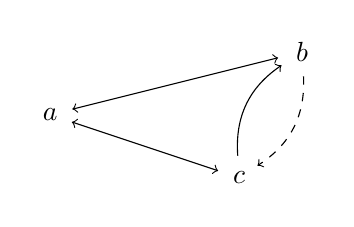
\begin{tikzpicture}
        [scale=.8,auto=right,every node/.style={circle}]
        \node (a) at (0, 2) {$a$};
        \node (b) at (4, 3) {$b$};
        \node (c) at (3, 1) {$c$};

        \draw[<->] (b) -- (a);
        \draw[<->] (a) -- (c);
        \draw (b) edge[bend left, ->, dashed] (c);
        \draw (c) edge[bend left, ->] (b);
    \end{tikzpicture}
\end{center}

\begin{center}
    \begin{tikzpicture}
        [scale=.8,auto=right,every node/.style={circle}]
        \node (a) at (0, 2) {$a$};
        \node (b) at (4, 3) {$b$};
        \node (c) at (3, 1) {$c$};

        \draw[<->] (b) -- (a);
        \draw[<->] (a) -- (c);
        \draw[<->] (c) -- (b);
    \end{tikzpicture}
\end{center}

\begin{center}
    \begin{tikzpicture}[every node part/.style={align=center}, 
    every path  shorten >= 1pt]
        \node (a) [draw, rounded rectangle] {$N_a c, N_b a$};
        \node (b) [draw, rounded rectangle, below left = of a] {
            \begin{tabular}[c]
                $N_a c, N_b a, N_c a$ \\
                $S_a c, S_c a$
            \end{tabular}
        };
        \node (c) [draw, rounded rectangle, below right = of a] {
            \begin{tabular}[c]
                $N_a b, N_a c, N_b a, N_b c$ \\
                $S_a b, S_b a$
            \end{tabular}
        };
        \node (d) [draw, rounded rectangle, below = of c] {
            \begin{tabular}[c]
                $N_a b, N_a c, N_b a, N_b c, N_c a$ \\
                $S_a b, S_a c, S_b a, S_b c, S_c a$
            \end{tabular}
        };
        \node (e) [draw, rounded rectangle, below = of b] {
            \begin{tabular}[c]
                $N_a b, N_a c, N_b a, N_b c, N_c a, N_c b$ \\
                $S_a b, S_a c, S_b a, S_c a, S_c b$
            \end{tabular}
        };
        \node (f) [accepting, draw, rounded rectangle, below = 5.8cm of a] {
            \begin{tabular}[c]
                $N_a b, N_a c, N_b a, N_b c, N_c a, N_c b$ \\
                $S_a b, S_a c, S_b a, S_b c, S_c a, S_c b$
            \end{tabular}
        };

        % \node (a) [draw, rounded rectangle, below = of d] {
        %     \begin{tabular}[c]
        %         $  N_a b, N_a c, N_b a, $ \\ $ S_a b, S_b a$
        %     \end{tabular}
        % };
        % \node (b) [draw, rounded rectangle, below = of a] {
        %     \begin{tabular}[c]
        %         $  N_a b, N_a c, N_b a, N_c a, N_c b$ \\ $ S_a b, S_a c, S_b a, S_c b, S_c a$
        %     \end{tabular}    
        % };
        % \node (c) [draw, accepting, rounded rectangle, below = of b] {
        %     \begin{tabular}[c]
        %         $  N_a b, N_a c, N_b a, N_b c, N_c a, N_c b$ \\ $ S_a b, S_a c, S_b a, S_b c, S_c b, S_c a$
        %     \end{tabular}    
        % };
        % \node (e) [right = of a] {$\ldots$};


        \path [->]
            (a) edge [] node [left] {$ac$} (b)
            (a) edge [] node [left] {$ba$} (c)
            (c) edge [] node [left] {$ac$} (d)
            (b) edge [] node [left] {$ba$} (e)
            (d) edge [] node [left] {$bc$} (f)
            (e) edge [] node [left] {$bc$} (f);
        %     (a) edge [out = 150, in = 210, loop] node[inner sep=2pt, align=left, sloped, above, pos = 0.3] {$ab, ba$} (a)
        %     (a) edge [] node [left] {$ac$} (b)
        %     (b) edge [] node [left] {$ab, ba, cb$} (c)
        %     (b) edge [out = 30, in = -30, loop] node[inner sep=2pt, align=left, sloped, above, pos = 0.7] {$ac, ca$} (b)
        %     (c) edge [out = 150, in = 210, loop] node[inner sep=2pt, align=left, sloped, above, pos = 0.3] {
        %         \begin{tabular}[c] 
        %         $ab, ac, bc,$ \\ $bc, ca, cb$
        %         \end{tabular}}
        %      (c)
        %     (d) edge [] node [left] {$ba$} (a)
        %     (d) edge [] node [right] {$ac$} (e);
    \end{tikzpicture}
\end{center}

%----------------------------------------------------------------------------------------
%	BIBLIOGRAPHY
%----------------------------------------------------------------------------------------

%----------------------------------------------------------------------------------------

\printbibliography[title={Bibliography}]

\end{document}
